% Плоский цикл.
\subsection{Плоские циклы}

\subsubsection{Понятие плоского цикла}

Векторизация программного контекста не может быть применена автоматически к коду произвольного вида.
В данном разделе определим подходящих для векторизации программный контекст специального вида -- плоский цикл -- и опишем его свойства.

\begin{figure}[ht]
\centering
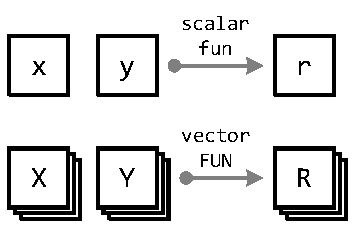
\includegraphics[width=0.4\textwidth]{./pics/text_4_flat/fun.pdf}
\caption{q}
\label{lab}
\end{figure}

На рис. 1 сверху представлена схема функции fun, которая получает на вход два аргумента x и y и на основании них формирует результат r.
Будем считать, что данная функция является чистой, то есть результат ее выполнения зависит только от значений x и y (например, отсутствуют побочные эффекты через глобальную память или операции ввода-вывода).
Идеология чистых вычислений берет свое начало из парадигмы функционального программирования [16], использование такого подхода открывает возможности для оптимизации программного кода, в частности для компиляторов.
Если рассмотреть вместо одного вызова функции fun несколько вызовов (w штук) с разными наборами входных параметров, то их можно трактовать как вызов некоторой функции FUN, входными параметрами которой являются векторы X и Y длины w, а выходным значением является вектор R также длины w.
В данном случае можно говорить, что функция FUN представляет собой реализацию векторизованной функции fun при ширине векторизации w (рис. 1 снизу).
В этом случае семантику функции FUN можно записать в виде

\begin{lstlisting}[caption={caption},label={label}]
for (int i = 0; i < w; ++i)
{
    r[i] = fun(x[i], y[i])
}
\end{lstlisting}

Цикл такого вида будем называть плоским циклом.
Определим свойства, присущие плоскому циклу.
Прежде всего условимся считать, что плоский цикл это цикл for, индуктивная переменная которого меняется от 0 до w - 1, где w -- ширина векторизации (например, при работе с набором инструкций AVX-512 и с вещественными значениями формата single precision ширина векторизации равна 16, то есть один zmm регистр вмещает 16 значений).
Во-вторых, будем считать, что внутри плоского цикла на i ой итерации все обращения в память (и вообще все обращения к глобальным данным) имеют вид a[i].
Такое ограничение гарантирует отсутствие конфликтов между итерациями по обращениям в память. Таким образом, итерации плоского цикла становятся независимыми между собой, а значит могут выполняться в произвольном порядке, в том числе и одновременно.

Плоские циклы, обладающие описанными свойствами, представляют собой удобный контекст для векторизации, и в большинстве случаев они могут быть векторизованы с помощью векторных инструкций AVX-512 с помощью перевода тела цикла в предикатное представление и замены скалярных инструкций векторными аналогами, реализованными с помощью функций-интринсиков [17,18].

Многие практические вычислительные задачи состоят из выполнения однотипных вычислений, применяемых к разным наборам данных, которые можно сгруппировать, трансформировав в плоский цикл, как это продемонстрировано на рис. 1 на примере функции fun.

Сложность векторизации тела полученного плоского цикла зависит от особенностей исходной функции fun.
Чем сложнее управление 
внутри тела векторизуемого плоского цикла, тем больше трудностей может возникнуть в процессе выполнения векторизации.
Для оценки сложности структуры векторизуемого тела цикла требуется построить граф потока управления данного цикла.

\subsubsection{Представление структуры тела плоского цикла в виде графа потока управления}

Граф потока управления (control flow graph, CFG) является одним из видов промежуточного представления программы, которые используются в частности для выполнения оптимизаций исполняемого кода [19].
Узлами данного графа являются линейные участки, состоящие из последовательностей инструкций, а ребрами -- передача управления между этими линейными участками [20].
Граф потока управления является логической структурой, отражающей параллелизм программы на уровне линейных участков.
Он активно используется компилятором для применения различных глобальных оптимизаций [21].

Кроме самой структуры графа потока управления для оптимизации программного кода важна статистическая информация об исполнении программы: количество выполнений различных линейных участков и данные о частоте переходов между ними.
Такая статистическая информация называется профилем исполнения, и для корректного проведения оптимизаций требуется правильным образом собирать и корректировать данный профиль [22].
Для векторизации программного кода профиль исполнения программы приобретает особенную важность, так как на эффективность векторизации сильно влияет даже структура векторных масок, которая сильно разнится при сравнении результатов, полученных при генерации случайных входных данных, и при использовании реальных данных расчетов [23].

Мы в качестве профиля исполнения приложения будем использовать данные только счетчики узлов и ребер, а также вероятности ребер. Обозначим некоторый узел CFG через v. Пусть в него входят несколько ребер, а также выходят несколько ребер (рис. 2).
Счетчиком произвольного ребра e будем называть количество переходов по этому ребру в процессе выполнения программы (значение счетчика ребра будем обозначать n(e)).
Счетчиком узла будем называть суммарное количество счетчиков всех входных ребер либо всех выходных ребер (для внутренних узлов CFG эти значения совпадают).
\begin{equation}
	n(v) = \sum_{e \in E_i(v)}{n(e)} = \sum_{e \in E_o(v)}{n(e)}
\end{equation}

Вероятностью ребра будем называть отношение счетчика данного ребра с счетчику узла, из которого это ребро выходит.
\begin{equation}
	\forall e \in E_o{v}: p(e) = \frac{n(e)}{n(v)}
\end{equation}

Построенный по телу плоского цикла граф потока управления с собранным профилем исполнения будем использовать для принятия решения о выборе методов векторизации программного контекста.

\begin{figure}[ht]
\centering
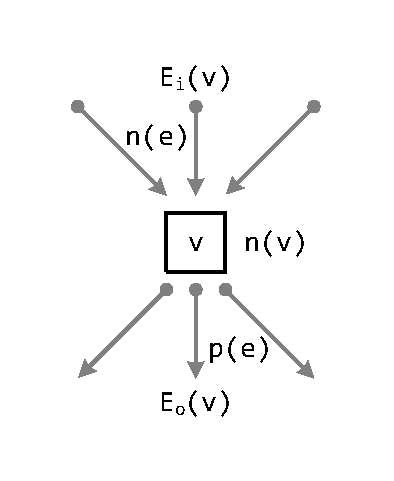
\includegraphics[width=0.4\textwidth]{./pics/text_4_flat/cfg.pdf}
\caption{q}
\label{lab}
\end{figure}
